
\documentclass{article}

% Load necessary packages
\usepackage[margin=1.5cm]{geometry}
\usepackage{natbib}
\usepackage{csquotes}
\usepackage{stmaryrd}
\usepackage{mathtools,amsfonts,amssymb,setspace}
\usepackage{amsmath}
\usepackage{amssymb}
\usepackage{array} 
\usepackage{caption}
\usepackage{subcaption}
\usepackage{ragged2e}
\usepackage{textgreek}
\usepackage{hyperref}
\usepackage{tikz}
\usepackage{tabularx}
\usepackage{adjustbox}
\usepackage{lipsum}
\usepackage{titlesec}

\begin{document}

\title{Operational long-term management of a salt cavern for industry targeted green H2 production}

\author{Robinson Beaucour \\Paris-Saclay University}

\maketitle


\begin{center}
    \includegraphics[width=0.4\textwidth]{03_Images/LITEN.png}
    \hspace{0.05\textwidth}
    \includegraphics[width=0.4\textwidth]{03_Images/LogoCS.png}
\end{center}

\begin{abstract}
    \small
    Hydrogen and its derivatives such as ammonia are increasingly important for reducing carbon emissions in sectors with limited alternatives. Large production systems are generally preferred to reduce costs and for those, advanced management is a cornerstone to the project economic viability.
    The present work explores the development of an Energy Management System for an industrial low-emission ammonia production platform. The latter is connected to the electrical grid and consists of 1.5 GW of renewable production units, around 500 MW of electrolyzers and storage facilities including especially a salt cavern for H2 storage. The long-term management of the salt cavern is decisive to enhance the profitability while satisfying industry related constraints such as the carbon content of the produced H2. The literature lacks in addressing both aspects simultaneously. 
    Methodological approaches to tackle the long-term management and industrial constraints are proposed and compared. For the considered platform, it is shown that a strategy based on precalculated cost functions in the long term horizon allows relative gains of 2.5\% with respect to a state-of-the-art short term management leading to an annual cost saving of approximately \$6.2 million in the platform operational expenses. This translates to a reduction of the gap between the state-of-the-art and the optimal \textit{a posteriori} solution by about 82\%.
\end{abstract}



\clearpage
\section{Introduction}
\label{Intro}

TEST TEST
\section{Context}

The utilization of hydrogen stands as a pivotal step towards combating climate change through the decarbonization of industrial processes, transportation and the seamless integration of variable renewable energy sources into the electricity grid \citep{shukla2022climate}.
Presently, there is a significant global upsurge in the demand for hydrogen, highlighting its increasing importance across various sectors \citep{iea_global_2022}. Especially for industry, hydrogen can be converted into ammonia in order to be primarily used for fertilizers. 
\\
With this rise in demand, low-emission hydrogen production is expected to grow from 1 to about 20 Mtons/year \citep{iea_global_2022} leading to a constant expansion of the pipeline of projects aiming at fostering low-emission hydrogen production. In order to reduce the specific production costs, gradually larger projects are announced with capacities already well exceeding 300MW planned in Germany, China and Australia \citep{iea_hydrogen_2023}.
\\
Concurrently, standards regarding the definiton of low-emission hydrogen are being discussed, initiating the need to anticipate new production constraints for the project holders. For instance, the \cite{green_hydrogen_organisation_green_2023} proposes to define a standard requiring that green hydrogen projects operate at less than 1 ton of CO2 emitted per ton of H2 produced taken as an average over a 12-months period.
\\

In pursuit of enhancing the competitiveness and integration of low-emission hydrogen within the broader energy landscape, extensive research has been undertaken. This integration marks a paradigm shift in scientific understanding with the emergence of smart energy systems \citep{lund_smart_2017}, which employ multiple energy vectors.
Hydrogen can be integrated into such systems mainly through electrolysis processes to boost power-to-gas production  while the waste heat from these processes can be valorized through district heating for e.g. \citep{guelpa_towards_2019}.
The literature presents studies of numerous multi-vector systems. \cite{gabrielli_optimal_2018} delved into the optimal design of energy systems encompassing both electricity and heat demands, thereby facilitating the integration of a substantial proportion of renewable electricity through hydrogen production and storage mechanisms.
\cite{haratyk_nuclear-renewables_2012} conducted an in-depth exploration of a nuclear-renewable energy system focusing on both hydrogen and electricity production, adressing particularly the utilization of electrolyzer partial and overload modes and hydrogen storage mechanisms to effectively balance the inherent variability of wind energy.
\\
Moreover, as planned for the announced projects \citep{iea_hydrogen_2023}, low-emission hydrogen production is generally associated to storage capacities and particularly large ones. The interest for large storage is also denoted in the literature in the field of power-to-gas-to-power. \cite{gabrielli_seasonal_2020} shed light on the immense potential of extensive hydrogen storage solutions, such as salt caverns, in mitigating CO2 emissions from energy grids characterized by high variable renewable energy production shares.
\cite{clerjon_matching_2019} uses an innovative signal decomposition approach \citep{CLERJON2022122799} to show that seasonal electricity storage is particularly difficult to ensure and the only economically viable solution appears to be H2 storage in salt caverns.\\

As stated beforehand, the future industrial green H2 production plant will be large and probably associated to large salt cavern. The latter means that an optimized operational management, i.e. an Energy Management Systems (EMS), should allow for consequent financial savings. However, this EMS will face the following challenges: 
\begin{itemize}
    \item The horizon of prediction of renewable productions does not exceed few days while the system is equipped with a storage which capacity exceeds weeks of production. This time-scale mismatch leads to the necessity of adding long-term management capabilities to the EMS.
    \item Within the industrial context, the green H2 must be produced respecting constraints such as CO2 content \citep{green_hydrogen_organisation_green_2023} or rate of production to match the low flexibility of downstream processes such as Haber-Bosch ammonia production reactor \citep{shamiri_modeling_2021}.
\end{itemize}
In the present work, an EMS that accounts for long-term management and industrial constraints is developed in order to evaluate the financial savings obtained on a large-scale plant.


\subsection{State-of-the-art}
The existing literature offers a rich array of methodologies for constructing EMS \citep{weitzel_energy_2018}. As summarized by \cite{alabi_strategic_2023}, the two advanced EMS methodologies that can cope with the dynamic variations of smart energy systems are Model Predictive Control (MPC) and Reinforcement Learning (RL). The latter approaches are illustrated by \cite{stoffel_evaluation_2023}, in the context of building energy management systems, who compared traditional reactive expert rules to model-free RL, MPC based on white-box, gray-box and black-box modeling and approximate MPC. While RL seems promising, there are still scientific challenges to overcome such as its lake of explicability, the effective management of specific constraints and the necessary consequent offline training on precise simulators. Those are probably the reasons why the studies that have probed the domain of EMS tailored specifically to hydrogen production in industrial settings are based on MPC.
\\
Noteworthy among these, \cite{klyapovskiy_optimal_2021} showcased the considerable potential of EMS in increasing the economic performance of industrial facilities reliant on hydrogen. Their approach involved the utilization of hydrogen and electricity, partially sourced from local renewables, emphasizing the pivotal role of EMS in optimizing such intricate energy systems, all executed within the framework of a Mixed-Integer Linear Programming (MILP) model. Expanding on this, their approach assesses energy management across four representative days, providing a planning horizon with a renewable production forecast of 24 hours. Such an approach however lacks the management of long term phenomena.
\\
Regarding EMS strategies including long term management but not in the field of hydrogen production, \cite{cuisinier_new_2022,cuisinier_impact_2023} presented a rolling horizon approach based on a MILP model that combines the short term, evaluated hourly, and the long term, evaluated at an arbitrarily longer interval.
The sole decision variable for the long term becomes the variation in the State of Energy (SOE) of the long-term storage, a thermal pit storage associated to district heating in their case. This variable is employed by Cost Functions (CF), which represent the operational cost of the system for a given time interval and for a variation of storage SOE. These CF are precalculated based on numerous MILP models over Representative Periods (RP) of the long term horizon.
\\

Based on the analysis of the state-of-the-art, none of the papers examined cope with industrial constraints such as maximal CO2 content of the produced H2 or minimal H2 rate of production. The most recent and advanced approaches for EMS tailored specifically to hydrogen production in industrial settings are based on hierarchical approaches, that may have difficulties to cope with such constraints. In the field of district heating, the methodological continuous approach of \cite{cuisinier_new_2022} is promising in order to both cope with the long term management of the salt cavern and these industrial constraints.


\section{System investigated and methods}
\subsection{Modeling approach} \label{Models}

The platform is modeled using a MILP formulation. The nomenclature of parameters and decision variables are described in \autoref{tab:system_parameters_and_DV}.
It uses the indice $sys$ for each type of system, with the set of indices for each type of system being described in \autoref{tab:system_description}.
Two renewable production systems are considered: photovoltaic (PV) and wind tubine (Wind). Five flow systems are considered: electricity consumed from global grid (ElecCons), electricity injected to the global grid (ElecInj), electricity curtailed from renewables (ElecCurt), $H_2$ sold from the local grid ($H_2$sold), $H_2$ bought or penalties ($H_2$pen).
Three converters are used, namely for renewable (Ren), electrolysers (Ely), compressors (Comp). Three storages are used, namely battery, pipeline, salt cavern (Cavern). In the remainder of the paper, decision variables of the MILP problem are written in bold while binary variables are written in lower case.\\
The MILP modeling for the renewable production, grid, converters, compressors and storage is rather common and thus described in \ref{app:model}. As detailed in \ref{app:model}, the grid, converters, compressors and storage sets of equations are respectively denoted \textit{F}, \textit{C}, \textit{K} and \textit{S}.

\begin{table*}
    \centering
    \tiny
    \caption{Parameters and decision variables}
    \begin{tabular}{|p{3.5cm}p{6.5cm}p{5cm}|}
    \hline
    \multicolumn{3}{|c|}{\textbf{(E) Renewable production}} \\[0.3cm]
$E_t^{(sys,power)}$                   &  Capacity factor at $t$ produced by $sys$                   & $ [MW/MW_c]$ \\ 
    $E^{(sys,capacity)}$                  & Capacity installed of $sys$                                 &  $[MW]$ \\
    $E^{(sys,CO_2)}$                      & $CO_2$ intensity of $sys$                                   & $[tCO_2/MWh]$ \\
    \multicolumn{3}{|c|}{\textbf{(F) Grid flow}} \\[0.3cm]
$F_t^{(sys,prices)}$                  & Price of $sys$ flow at $t$                     & $[\$/MWh]$ or $[\$/tH_2]$ \\
    $F^{(sys,max/min)}$                   & Max/Min flow of $sys$                          & $ [MW]$ or $ [tH_2/h]$ \\
    $F^{(sys,sens)}$                      & Sens of $sys$ : 1 if input, -1 if output       &  \\
    $F^{(sys,CO_2)}$                      & $CO_2$ intensity of $sys$                      & $[tCO_2/MWh]$ or $[tCO_2/tH_2]$ \\[0.3cm]
$\textbf{F}_\textbf{t}^{\textbf{(sys,flow)}}$           & Flow of $sys$ at $t$                     & $[MW]$ or $[tH_2/h]$ \\
    $\textbf{F}_\textbf{t}^{\textbf{(sys,cost)}}$           & Cost of $sys$ flow at $t$                & $[\$]$ \\
    $\textbf{F}_\textbf{t}^{\textbf{(sys,CO$_2$)}}$            & $CO_2$ emits by $sys$ flow at $t$        & $[tCO_2]$ \\[0.3cm]
    \multicolumn{3}{|c|}{\textbf{(C) Converter}} \\[0.3cm]
$C^{(sys,eff)}$           & Conversion efficiency of $sys$                         & $[-]$ \\
    $C^{(sys,max/min)}$       & Max/Min conversion of $sys$                            & $[MW]$ \\[0.3cm]
$\textbf{C}_\textbf{t}^{\textbf{(sys,in)}}$             & Input flow of $sys$ converter at $t$       & $[MW]$ \\
    $\textbf{C}_\textbf{t}^{\textbf{(sys,out)}}$            & Output flow of $sys$ converter at $t$      & $[MW]$ \\[0.3cm]
    \multicolumn{3}{|c|}{\textbf{(K) Compressor}} \\[0.3cm]
$K^{(sys,coef)}$          & Coefficient conversion of $sys$                            & $[MW/(tH_2/h)]$ \\
    $K^{(sys,max/min)}$       & Max/Min flow of $sys$                                      & $[MW]$ \\[0.3cm]
$\textbf{K}_\textbf{t}^{\textbf{(sys,elec)}}$           & Electricity of $sys$ compressor at $t$       & $[MW]$ \\
    $\textbf{K}_\textbf{t}^{\textbf{(sys,H$_2$)}}$            & $H_2$ flow through $sys$ compressor at $t$   & $[MW]$ \\[0.3cm]
    \multicolumn{3}{|c|}{\textbf{(S) Storage}} \\[0.3cm]
    $S^{(sys,ChargeEff)}$             & Charge efficiency of $sys$                         & $[-]$ \\
    $S^{(sys,Disc.Eff)}$              & Discharge efficiency of $sys$                      & $[-]$ \\
    $S^{(sys,StatLosses)}$            & Static Losses of $sys$                             & $[-]$ \\
    $S^{(sys,ChargeMax)}$             & Max charge of $sys$                                & $ [MW]$ or $ [tH_2/h]$ \\
    $S^{(sys,Disc.Max)}$              & Max discharge of $sys$                             & $ [MW]$ or $ [tH_2/h]$ \\
    $S^{(sys,Max/MinSOE)}$            & Max/MIN SOE of $sys$                               & $[-]$ \\
    $S^{(sys,SOEini)}$                & SOE initial of $sys$                               & $[-]$ \\
    $S^{(sys,Capacity)}$              & Capacity of $sys$                                  & $[tH_2]$ or $[MWh]$ \\[0.3cm]
    $\textbf{S}_\textbf{t}^{\textbf{(sys,SOE)}}$        & SOE of $sys$ storage at $t$                        & $[-]$ \\
    $\textbf{S}_\textbf{t}^{\textbf{(sys,ChargeFlow)}}$ & Charge flow of $sys$ storage at $t$                    & $[MW]$ \\
    $\textbf{S}_\textbf{t}^{\textbf{(sys,Disc.Flow)}}$  & Discharge flow of $sys$ storage at $t$                 & $[MW]$ \\
    $\textbf{S}_\textbf{t}^{\textbf{(sys,Flow)}}$       & Flow of $sys$ storage at $t$                           & $[MW]$ \\
    $\textbf{s}_\textbf{t}^{\textbf{(sys,state)}}$      & state of $sys$ storage at $t$ : 0 if charging else 1   &  \\[0.3cm]
    \multicolumn{3}{|c|}{\textbf{(L) Electrolyser}} \\[0.3cm]
    $L^{(k,max/min)}$                   & Max/Min power of the $k^{th}$ electrolyser                                        & $[MW]$ \\
    $L^{(k,AuxBase)}$                   & Base electricity consumption of the $k^{th}$ electrolyser                         & $[MW]$ \\
    $L^{(k,AuxMarg)}$                   & Marginal electricity consumption rate of the $k^{th}$ electrolyser                &  \\
    $L_i^{(k,elec)}$                    & electricity $i^{th}$ operating point of the $k^{th}$ electrolyser                 & $[MW]$ \\
    $L_i^{(k,H_2)}$                     & $H_2$ flow $i^{th}$ operating point of the $k^{th}$ electrolyser                  & $[tH_2/h]$ \\[0.3cm]
    $\textbf{L}_\textbf{t}^{\textbf{(k,elec)}}$           & Electricity consumption of the $k^{th}$ electrolyser at $t$ for $H_2$             & $[MW]$ \\
    $\textbf{L}_\textbf{t}^{\textbf{(k,H$_2$)}}$            & $H_2$ flow production of the $k^{th}$ electrolyser at $t$                         & $[tH_2/h]$ \\
    $\textbf{L}_\textbf{t}^{\textbf{(k,total)}}$          & Total electricity consumption of the $k^{th}$ electrolyser at $t$                 & $[MW]$ \\
    $\textbf{l}_\textbf{t}^{\textbf{(k,state)}}$          & State of the $k^{th}$ electrolyser at $t$ : 1 if turnd on else 0                  & $[MW]$ \\[0.3cm]
    \multicolumn{3}{|c|}{\textbf{Global parameters}} \\[0.3cm]
    $M^{(CO_2)}$                    & Maximum hourly $CO_2$ intensity of $H_2$ sold                                         & $[tCO_2/tH_2]$ \\
    $m^{(H_2)}$                     & Minimum hourly $H_2$ sold quantity                                                    & $[tH_2/h]$ \\
    $\Delta$                        & Duration of rolling constraints                                                       & $[h]$ \\
    $\delta_t$                      & Duration of instant $t$                                                               & $[h]$ \\
    $N_{ely}$                       & Number of electrolysers modules                                                       & \\
    \hline     
    \end{tabular}
    \label{tab:system_parameters_and_DV}
\end{table*}

\clearpage
\appendix

\section{MILP models} \label{app:model}
The present Appendix describes the MILP modeling for the renewable production, grid, converters, compressors and storage.
\subsection{Renewable production} \label{Renewable_production}

PV and wind production are modeled with capacity factor time series considered as inputs for the optimization problem. Thus, no decision variables are related to renewable production.

\subsection{Grid Flow} \label{Grid_Flow} \label{eq:F}
Local electricity grid can consume (related to \textit{ElecCons}) or inject (related to \textit{ElecInj}) electricity from/to the global electricity grid. The local $H_2$ grid can sell $H_2$ (related to \textit{$H_2$sold}). If the platform does not satisfy production or $CO_2$ constraints (see Section \ref{specific_constraints}), it can "buy" expensive external green $H_2$ (related to \textit{$H_2$pen}). \textit{$H_2$pen} can be interpreted as a penalty to prevent unfeasabilty during the platform operation. Equations (\ref{eq:F1}) and (\ref{eq:F2}) set hourly cost and $CO_2$ emissions for each flow, system and instant. Equation (\ref{eq:F3}) sets flow constraints related to infrastructures limitation.

\begin{equation} \tag{F.1} \label{eq:F1}
    \textbf{F}_\textbf{t}^{\textbf{(sys,cost)}} = F^{(sys,sens)} \cdot F_t^{(sys,prices)} \cdot \textbf{F}_\textbf{t}^{\textbf{(sys,flow)}}
\end{equation}
\begin{equation} \tag{F.2} \label{eq:F2}
    \textbf{F}_t^{(sys,CO2)} = F^{(sys,CO_2)} \cdot \textbf{F}_\textbf{t}^{\textbf{(sys,flow)}}
\end{equation}
\begin{equation} \tag{F.3} \label{eq:F3}
    F^{(sys,min)} \leq \textbf{F}_\textbf{t}^{\textbf{(sys,flow)}} \leq F^{(sys,max)}
\end{equation}


\section{MILP tolerance} \label{app:MILP}
In this Appendix, the impact of the modeling of the electrolysers with SOS2 variables is evaluated. The objective is to check that the operating points of the electrolysers on the obtained results do not deviate from the operating curve of \autoref{fig:ely_operating_range}. The gap between operating point given by the EMS and operating curve is calculated with Equation (\ref{eq:L2}). \autoref{fig:ely_gap} provides a visual representation of the gap, demonstrating that only a few operating points are significantly outside the allowed range. 
\begin{equation*}
     \text{Gap}_t = \textbf{L}_\textbf{t}^{\textbf{(k,elec)}} \cdot \alpha_i^{(k)} - \textbf{l}_\textbf{t}^{\textbf{(k,state)}} \cdot \beta_i^{(k)} - \textbf{L}_\textbf{t}^{\textbf{(k,H$_2$)}}
\end{equation*}
Despite minor deviations, the solutions remain close to the operating curve, attesting to the effectiveness and reliability of the MILP-based optimization approaches in achieving near-optimal EMS operation while adhering to constraints.\\

It is worth mentioning here that for all the results obtained, the solver used is CPLEX 22.1.0 and the relative gap between the solution returned and the optimal solution is notably small, with a value of 0.01 for both the \textit{Myopic} and \textit{Price Signal} approaches and an even smaller value of 0.001 for the \textit{Multiple RP-CF approach}. The reduced tolerance for RP-CF can be attributed to the consideration of long-term cost, requiring higher precision in the optimization process.

\begin{figure}
    \centering
    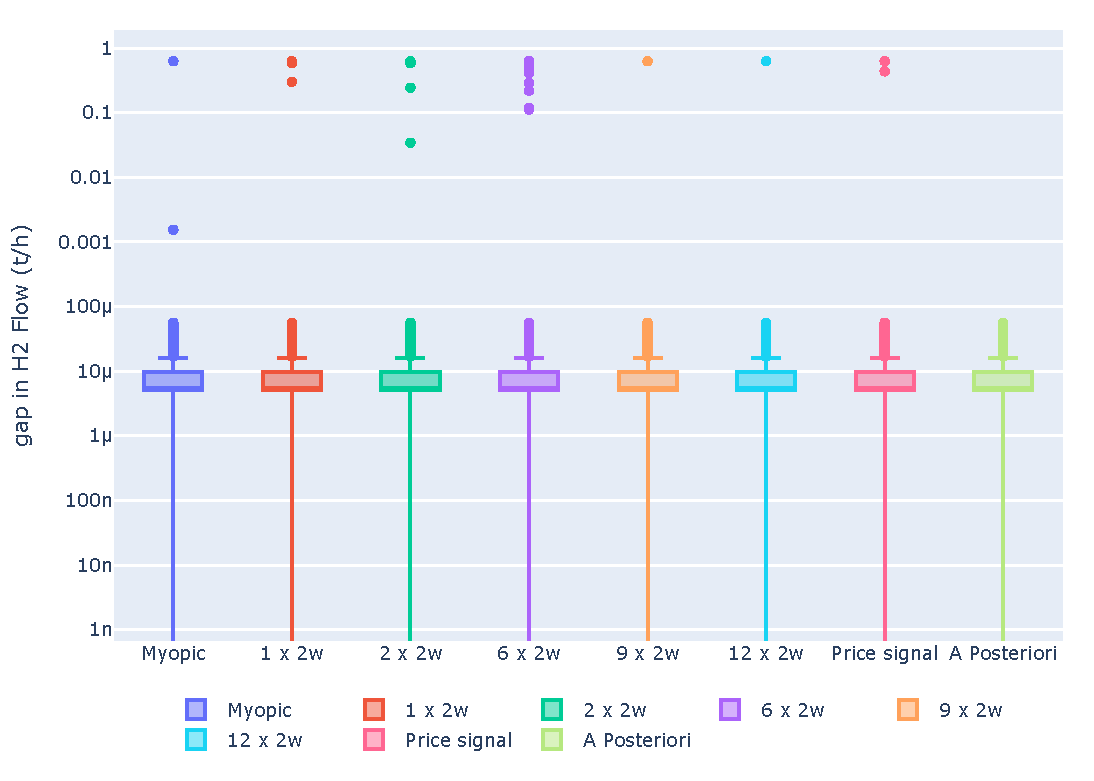
\includegraphics[width=10cm]{02_Appendix/MILP_tolerance_boxplot.pdf}\\
    \caption{Absolute gap between operation range of electrolyser and operating point of the EMS}
    \label{fig:ely_gap}
\end{figure} 

\bibliographystyle{elsarticle-num-names}
\bibliography{ref}

\end{document}
